\chapter{Materiais e Métodos}

Neste capítulo são descritos os procedimentos e materiais adotados no trabalho. Inicialmente, tem-se uma breve caracterização dos projetos selecionados nas organizações citadas na seção 3.4 inerente ao capítulo sobre metodologia. Posteriormente, são descritas todas as ferramentas utilizadas para coleta de dados. Por fim, são apontadas as atividades executadas neste estudo de acordo com o procedimento técnico pesquisa-ação.

\section{Projetos selecionados na CGDF}

Pelo fato de o presente trabalho propor um \textit{framework} que reúne as práticas complementares e fundamentais da verificação de \textit{software} (testes e inspeções), bem como conceitos da VBSE, procurou-se selecionar produtos que possuem impacto significativo na missão da CGDF e que não possuíam tais práticas sendo utilizadas no seu processo de desenvolvimento.

\subsection{Portal da Transparência do Distrito Federal}

O primeiro produto selecionado foi o Portal da Transparência do Distrito Federal (www.transparencia.df.gov.br). Esta é uma ferramenta de participação da sociedade no controle das ações do Governo. Dentre as informações disponibilizadas pelo portal, destacam-se informações sobre a contabilidade do Governo do Distrito Federal, tais como: instrumentos de planejamento, receitas públicas arrecadadas pelo Governo, despesas públicas realizadas pelo Estado, licitações dos órgãos do Governo do Distrito Federal e remuneração dos servidores.

O Portal da Transparência do Distrito Federal já se encontra em sua terceira versão. De acordo com a CGDF, a reformulação do Portal, culminando em sua terceira versão, fez com que os acessos aumentassem em cerca de 34\% em dezembro de 2016 e janeiro de 2017 em relação ao mesmo período no ano passado. A quantidade de usuários únicos no site, nesse intervalo, passou de 174.232 para 234.653 de acordo com o último levantamento.

A terceira versão do Portal foi concebida de forma a facilitar a navegação do usuário, bem como a compreensão dos dados disponibilizados. Adicionalmente, procurou-se desenvolver uma solução escalável, de forma que os dados pudessem ser utilizados por outros sistemas.

Desde o início da concepção arquitetural da terceira versão do Portal foram adotadas tecnologias modernas no âmbito do desenvolvimento de aplicações \textit{web}. Basicamente, adotou-se o \textit{framework AngularJS} para elaboração da aplicação cliente e o \textit{Spring Framework}, desenvolvido em linguagem Java, para construção da API \textit{REST (Representational State Transfer)} que é utilizada como \textit{backend}. A seguir, tem-se uma figura que exibe a página inicial do Portal e outra que exibe um esquema da arquitetura do Portal.

\begin{figure}[h]
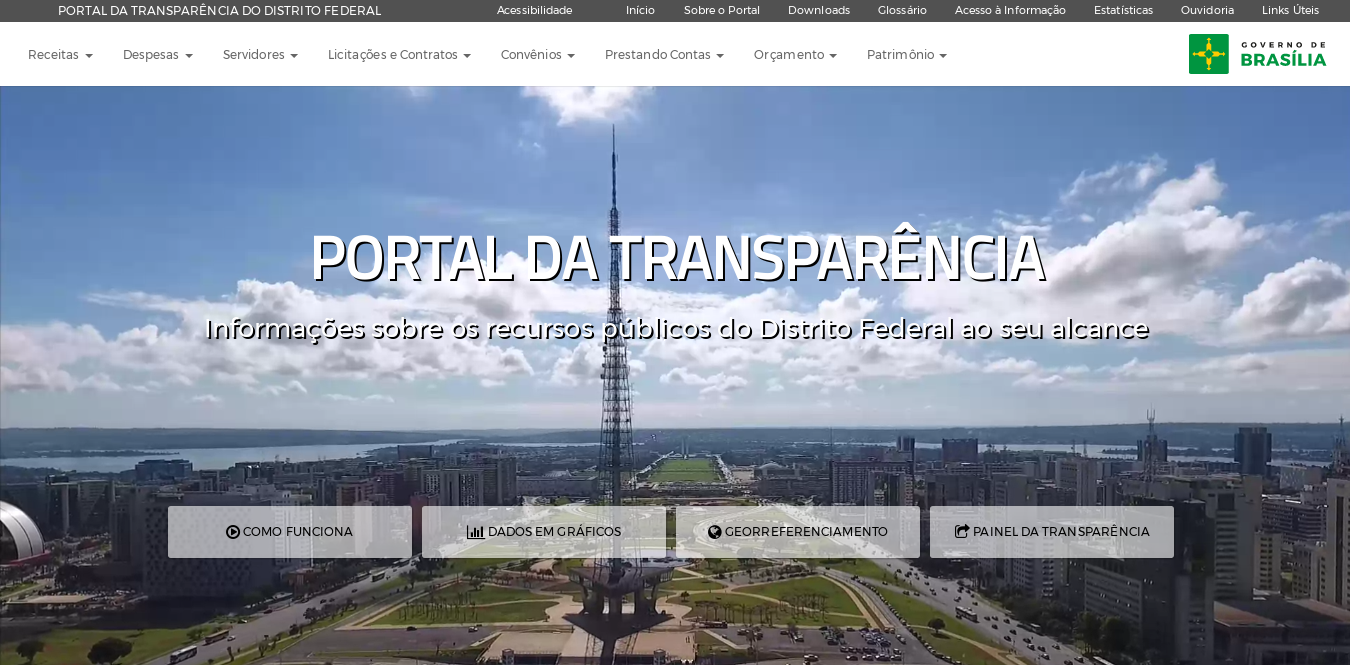
\includegraphics[width=\textwidth]{figuras/portalTransparencia.png}
\caption{Página inicial - Portal da Transparência do Distrito Federal}
\end{figure}

\begin{figure}[h]
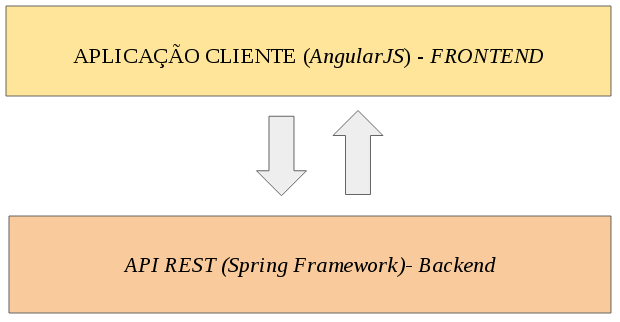
\includegraphics[width=\textwidth]{figuras/arquiteturaPortal.png}
\caption{Esquema Arquitetural - Portal da Transparência do Distrito Federal}
\end{figure}

O Portal passa por constantes evoluções. Todos os dias dados são atualizados e novas funcionalidades são incorporadas em uma periodicidade de 3 semanas, tempo de duração de uma \textit{sprint} no processo de desenvolvimento da COTEC. Assim, percebeu-se a importância de utilizar concisamente práticas da verificação de \textit{software} para melhorar a qualidade do Portal.

\subsection{Sistema de Ouvidoria do Distrito Federal}

O segundo produto selecionado foi o Sistema de Ouvidoria do Distrito Federal (www.ouv.df.gov.br). A Ouvidoria é um espaço que organiza a comunicação entre o cidadão e o governo, favorecendo a participação popular, a transparência e o aperfeiçoamento da prestação dos serviços públicos.

Como parte da estrutura da CGDF, existe a Subcontroladoria denominada Ouvidoria-Geral do DF. Esta é responsável pela coordenação dos trabalhos das Ouvidorias Especializadas - localizadas em cada órgão do Governo do Distrito Federal.

O sistema de ouvidoria também passou por uma reformulação, sendo que já se encontra em sua segunda versão. Dentre as melhorias realizadas na navegação, foram incluídas novas funcionalidades que fornecem maior transparência ao cidadão durante o atendimento de sua manifestação.

Assim como no Portal da Transparência, durante a concepção arquitetural da segunda versão do sistema de ouvidoria foram adotadas tecnologias modernas para o desenvolvimento. A camada de apresentação também utiliza o \textit{framework AngularJS} e a camada \textit{backend} foi construída utlizando a linguagem \textit{CSharp} seguindo as diretrizes do estilo arquitetural MVC (\textit{Model, View, Controller}) e também, do estilo de desenvolvimento DDD (\textit{Domain Driven Design}).

O DDD, por sua vez, é uma abordagem que se alinha concisamente às ideias apresentadas pela VBSE, pois basicamente, um dos aspectos mais destacados nesta abordagem é que o código produzido deve estar bem alinhado ao negócio. Este conceito, se utilizado corretamente, favorece a reutilização pois os blocos de construção facilitam o aproveitamento de um mesmo conceito de domínio ou um mesmo código em vários lugares \cite{ddd}. Adicionalmente, com um modelo bem feito e organizado, as diversas partes de um sistema interagem sem que haja muita dependência entre os módulos ou classes de objetos de conceitos distintos, acarretando em um quadro mínimo de acoplamento.

Embora tenham sido feitas boas escolhas quanto às tecnologias e arquitetura, o sistema de ouvidoria também necessita de um controle de qualidade mais rigoroso, visto que assim como o Portal, também passa por constantes evoluções. A figura a seguir exibe a página inicial do Sistema de Ouvidoria do Distrito Federal.

\begin{figure}[h]
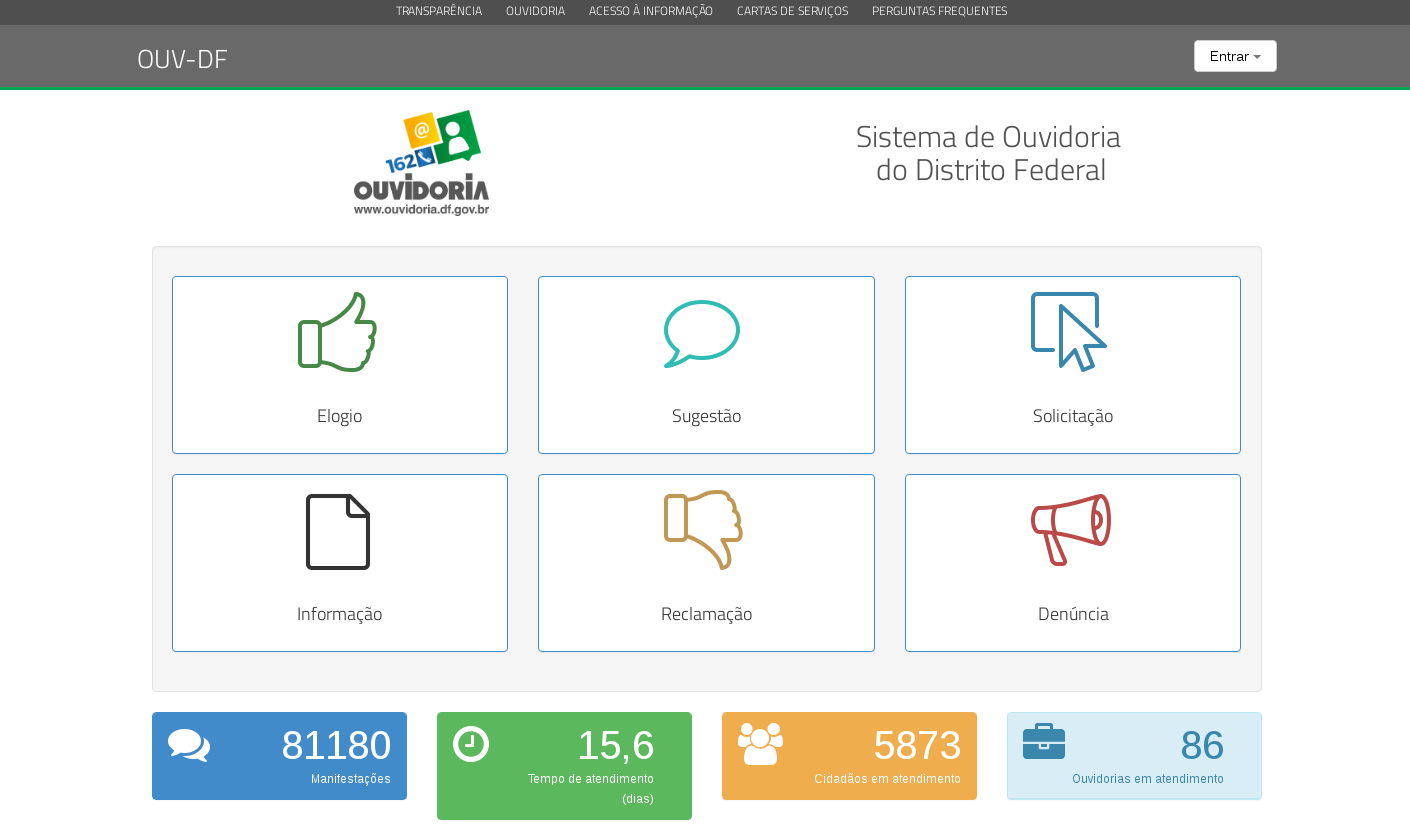
\includegraphics[width=\textwidth]{figuras/sistemaOuvidoria.png}
\caption{Página inicial - Sistema de Ouvidoria do Distrito Federal}
\end{figure}

\section{Projeto selecionado no Laboratório Fábrica de \textit{Software}}

\subsection{Sistema de Perícia Médica}

O Laboratório Fábrica de \textit{Software} possui atualmente uma parceiria com uma instituição privada que, por motivos de políticas de sigilo, não terá sua identidade revelada neste trabalho. Contudo, a mesma será tratada como Instituição X.

A Instituição X é uma empresa que promove processos seletivos e aplica diversos tipos de exames no Brasil. Determinados processos seletivos organizados pela empresa necessitam de uma etapa adicional para a realização da perícia médica nos candidatos classificados para as fases posteriores. Atualmente, todo este processo é manual, envolvendo o preenchimento de fichas e um exaustivo trabalho para passar todos estes dados para o meio digital.

Tendo em vista esta oportunidade de negócio, a Instituição X solicitou o desenvolvimento de um sistema para automatizar o registro e compilação dos dados inerentes à perícia médica ao Laboratório Fábrica de \textit{Software}.

A solução proposta pelo Laboratório Fábrica de \textit{Software} envolve a elaboração de duas aplicações que funcionarão de forma conjunta. Há uma aplicação \textit{web}, sendo desenvolvida em linguagem de programação \textit{CSharp}, seguindo o estilo arquitetural MVC. Nesta aplicação, a área de negócio pode montar fichas personalizadas de perícia médica para os diversos editais que são publicados. Adicionalmente, a aplicação \textit{web} recebe todos os dados enviados pela segunda aplicação, que é \textit{mobile} e esta foi projetada para ser utilizada nos locais de realização da perícia médica. A aplicação \textit{mobile} também está sendo desenvolvida em linguagem \textit{CSharp} e também segue as diretrizes do estilo arquitetural MVC.

A equipe de desenvolvimento do sistema de perícia médica também relatou a necessidade que possuíam de implementar um controle mais rigoroso da qualidade. Adicionalmente, a equipe também mencionou dificuldades na elaboração de testes unitários para a aplicação \textit{mobile}. Assim, o projeto caracterizou-se como uma excelente oportunidade para aplicação do \textit{framework} proposto por este trabalho.